% Indicate the main file. Must go at the beginning of the file.
% !TEX root = ../main.tex

%----------------------------------------------------------------------------------------
% EINLEITUNG
%----------------------------------------------------------------------------------------

\label{Chapter3} % Change X to a consecutive number; for referencing this chapter elsewhere, use \ref{ChapterX}

%----------------------------------------------------------------------------------------
% SECTION 1
%----------------------------------------------------------------------------------------

\chapter{Theoretische Grundlagen} % Main chapter title

In diesem Kapitel werden die theoretischen Grundlagen vorgestellt, die für das Verständnis dieser Arbeit notwendig sind. Zunächst werden Git und GitHub vorgestellt. Danach folgen die spezifischen Techniken, welche diese Systeme verwenden. Anschliessend werden die Projektmodule und deren Unterschiede zu Open Source Projekten erläutert. Zusätzlich wird das Tool GitGauge vorgestellt und dessen Architektur beschrieben.

\label{Chapter2} % Change X to a consecutive number; for referencing this chapter elsewhere, use \ref{ChapterX}

%----------------------------------------------------------------------------------------
% SECTION 1
%----------------------------------------------------------------------------------------

\section{Git \& Github}
Die Nutzung eines Versionskontrollsystems (VCS - version control system) ist ein zentrales Element der Softwareentwicklung. Mit einem VCS können Änderungen am Sourcecode nachverfolgt und bei Bedarf eine frühere Version des Projekts wiederhergestellt werden. Die Nutzung eines VCS ermöglicht ausserdem, dass mehrere Entwickler parallel am gleichen Code arbeiten können, indem die Änderungen inklusive deren Urheber sowie Zeitpunkt festgehalten werden. \parencite{noauthor_informationen_2025} 

Mit der Nutzung einer verteilten Versionsverwaltung (DVCS - distributed version control system), wird kein zentrales Repository mehr verwendet. Jeder Entwickler verfügt über eine Kopie des Projektes inklusive des gesamten Projektverlaufs. Änderungen können lokal implementiert werden. Eine Verbindung zum Server wird nur für das Synchronisieren von Änderungen notwendig. \parencite{noauthor_informationen_2025} 

Git ist heute das am meisten verbreitete DVCS-System. Es wurde von Linus Torvalds für die Entwicklung des Linux-Kernels entwickelt. \parencite{zack_git_2018} Git bezeichnet ein Projekt als ein Git-Repository, wobei der Verlauf als eine Reihe von Snapshots (Commits) modelliert wird. Diese Commits sind in unterschiedlichen Branches organisiert, welche die parallele Entwicklung ermöglichen. Die Verwendung von Branches ermöglicht die parallele Entwicklung von Bugs, neuen Features etc., ohne dass es zu gegenseitigen Beeinträchtigungen kommt. Diese unterschiedlichen Branches werden anschliessend gemerged. 

Mit dem Erfolg von Git entstanden Dienste und Anbieter, welche Git-Repositories online zur Verfügung stellen und zusätzliche Kollaborationstools anbieten. Github ist der bekannteste und auch am meisten verwendete Hosting-Dienst. Auf Github können Entwickler ihr Git-Repository hosten, Änderungen vorschlagen und diskutieren, Fehler (Issues) tracken. Github bietet eine Weboberfläche, welche für das Einsehen des Codes, aber auch für das Erstellen von Pull Requests und Issues verwendet werden kann. Zusätzlich kann der CI/CD-Prozess direkt mittels Github Actions abgebildet werden. \parencite{noauthor_informationen_2025}  

\section{Pull Request} 
Ein Pull Request ist ein Vorschlag, Änderungen von einem Branch oder Fork in einen anderen Branch zusammenzuführen. In einem typischen Entwicklungsworkflow erstellt der Entwickler für eine Änderung einen neuen Branch, committet dort seine Arbeit und erstellt anschliessend einen Pull Request. Ein Pull Request enthält dabei die durchgeführten Codeänderungen sowie eine Beschreibung zur Änderung. Die Unterschiede (Diffs) zwischen Quell- und Zielbranch werden dabei übersichtlich aufgezeigt \parencite{noauthor_about_nodate}.

Pull Requests spielen für den Code-Review und die Diskussion innerhalb des Entwicklungsprozesses eine wichtige Rolle. So bietet ein Pull Request eine Basis zur Diskussion, indem Teammitglieder den Code begutachten, kommentieren und auch Änderungen vorschlagen können \parencite{atlassian_pull_nodate}. Viele Entwicklerteams richten daher verbindliche Review-Prozesse ein, bei denen ein Pull Request (PR) erst dann gemergt werden kann, wenn dieser von mindestens einer Person genehmigt wurde \parencite{jiang_how_2022}.

Durch das Konfigurieren von automatischen Checks mittels CI/CD können sowohl Anforderungen an die Softwarequalität (zum Beispiel durch das automatisierte Ausführen von Tests oder statischen Codeanalysen) als auch an den Entwicklungsprozess automatisiert überprüft werden \parencite{kinsman_how_2021}. Dazu gehört beispielsweise die Überprüfung, ob alle Commits mit einem Signed-off-by versehen sind, was in vielen Projekten zur Einhaltung des Developer Certificate of Origin (DCO) verpflichtend ist \parencite{holtgrave_attributing_2025}. Diese Massnahmen stellen sicher, dass sowohl die technische Qualität des Codes als auch rechtliche Rahmenbedingungen eingehalten werden, bevor ein Pull Request gemergt wird \parencite{noauthor_about_nodate}. 

\subsection{Git Squashing}
\label{sec:GitSquashing}
Mit \textit{Git Squashing} wird die Praxis bezeichnet, mehrere Commits zu einem Commit zusammenzuführen, bevor diese in den Zielbranch gemerged werden. Dies kann entweder manuell durch ein interaktives Rebase über die Git-Kommandozeile oder automatisch erfolgen, indem beim Mergen des Pull Requests die Option \textit{Squash commits} ausgewählt wird. \parencite{noauthor_git_nodate} Je nach Plattform kann die Option zum automatischen Squashen von Commits beim Mergen des Pull Requests unterschiedlich bezeichnet sein \parencite{noauthor_about_nodate} \parencite{noauthor_squash_nodate}. \\
Daraus ergibt sich, dass alle Änderungen eines Feature-Branches im Zielbranch zusammengeführt werden, ohne die gesamte Historie zu übernehmen. Oftmals dient dies dazu, die Lesbarkeit des Projektverlaufs zu verbessern oder fehlerhafte Commits auszublenden \parencite{codoban_comparative_2015}. Darüber hinaus kann das Reverten von Commits erleichtert werden, da eine flache Git-Historie, die nur eine zusammengefasste Reihe von Commits enthält, beim Zurücksetzen von Änderungen Vorteile bietet \parencite{just_switching_2016}.

Nachteil ist der Verlust von Informationen über die schrittweise Entwicklung eines Features. Die Commits der jeweiligen Feature-Entwicklung und deren Nachrichten gehen verloren, was die Transparenz des Entwicklungsprozesses einschränkt.

\section{Pull Request Latency}
\label{sec:PullRequestDauer}
Es existieren bereits diverse Studien, die sich mit der Analyse von Pull Requests befassen. In der Literatur werden verschiedene Faktoren untersucht, die die Dauer von Pull Requests beeinflussen. Zusammenfassend kommen die Studien zum Schluss, dass die Pull Request Laufzeit von verschiedenen Faktoren, wie der Diskussion, Reputation des Erstellers, Team-Auslastung, erster menschlicher Reaktion und Continuous Integration abhängig ist. Es existieren jedoch widersprüchliche Aussagen bezüglich der Abhängigkeit der Laufzeit von der PR-Grösse. \parencite{yu_wait_2015}\parencite{hasan_understanding_2023}\parencite{kudrjavets_small_2022}\parencite{bernardo_studying_2018}

Ein Beispiel ist das Paper von Yue Yu u.a.\parencite{yu_wait_2015}, welches  mittels linearer Regressionsmodelle relevante Faktoren bei GitHub-Projekten analysiert hat. Die Resultate der Untersuchung zeigen, dass Faktoren wie die Grösse – definiert als die Anzahl der Änderungen des Pull Requests – oder die Länge der Diskussion über den Pull Request die Laufzeit beeinflussen. Des Weiteren wurde ein Zusammenhang zwischen der Reputation des Stellers und der Dauer nachgewiesen. Darüber hinaus wurde ein Zusammenhang zwischen der Grösse des Teams, der Auslastung - definiert als Anzahl offener Pull Requests - sowie der Zeit bis zur ersten menschlichen Reaktion auf den Pull Request festgestellt. Zusätzlich wurde gezeigt, dass CI-Faktoren einen signifikanten Einfluss haben, wie beispielsweise das Warten auf automatisierte Tests.~\parencite{yu_wait_2015}

Das Paper von Kazi Amit Hasan u.a.\parencite{hasan_understanding_2023} befasst sich spezifischer mit der ersten Reaktion auf einen Pull Request anhand von Open Source Projekten. In diesem Zusammenhang sind Reaktionen definiert in Form eines Kommentars auf einen Pull Request oder eines Code-Review-Kommentars auf einen Pull Request. Es wurde festgestellt, dass die erste Antwort eines Bots kaum Auswirkungen auf die Dauer hat, die erste Antwort eines Menschen jedoch einen grossen Einfluss hat. Die Dauer der ersten menschlichen Reaktion ist in der Hälfte der Fälle auf neun Faktoren zurückzuführen. Diese neuen Faktoren sind die Länge der Beschreibung, die Anzahl Commits, die Anzahl bearbeiteter Files, die Anzahl geänderter Codezeilen, die Anzahl hinzugefügter Codezeilen,  ob eine Person auf dem Pull Request markiert wurde, die Anzahl offener Pull Requests, die Anzahl der bisherigen Pull Requests des Entwicklers und der Anteil der Teammitglieder, mit denen der Entwickler in den letzten drei Monaten interagiert hat. Insbesondere Pull-Requests, die beim Eröffnen eine längere Beschreibung und komplexere Code-Änderungen haben, dauert die erste menschliche Reaktion länger. Ebenfalls stellten sie einen Zusammenhang bezüglich der Auslastung, also den offenen PRs und der ersten Interaktion fest. Ein weiteres Resultat ihrer Recherche zeigte auf, dass Verfasser mit weniger Erfahrung (Anzahl erfasster PRs) und fehlende Interaktionen mit Projektmitgliedern ebenfalls zu längeren ersten menschlichen Reaktionen führen kann.\parencite{hasan_understanding_2023} 

Beide oben beschriebenen Studien stellen einen Zusammenhang zwischen der Grösse eines Pull Requests und dessen Dauer fest \parencite{yu_wait_2015}\parencite{hasan_understanding_2023}. Die Studie von Gunnar Kudrjavets, Nachiappan Nagappan und Ayushi Rastogi  \parencite{kudrjavets_small_2022}, die sich spezifisch mit dieser Thematik befasst, gelangt zu dem Schluss, dass kein Zusammenhang zwischen diesen beiden Aspekten festgestellt werden kann.

Das Paper von João Helis Bernardo, Daniel Alencar Da Costa und Uirá Kulesza \parencite{bernardo_studying_2018} fand heraus, dass Projekte, die Continuous Integration eingeführt haben, danach Pull Requests mit längeren Laufzeiten hatten.


\section{Pull Request Akzeptanz}
Die Akzeptanz eines Pull Requests bestimmt, ob ein Pull Request gemerged oder abgelehnt (rejected) wird. Über die Einflussfaktoren der Akzeptanz von Pull Requests existieren bereits mehrere Studien.
So zeigen diverse Untersuchungen, dass die Akzeptanz eines Pull Requests von mehreren technischen als auch sozialen Faktoren abhängig ist \parencite{gousios_exploratory_2014}. \
Eine Studie, die über 40'000 Pull Requests in Projekten mit unterschiedlichen Programmiersprachen (Java, Python, C etc.) analysierte, stellte fest, dass die Code-Qualität nur einen geringen Einfluss auf die Akzeptanzrate hat \parencite{kuhejda_pull_2023}.

Die Grösse eines Pull Requests (Umfang der Code-Änderungen) ist ein technisches Merkmal, das in der Literatur häufig erwähnt wird. Hierzu gibt es in der Forschung unterschiedliche Ergebnisse. So stellte eine Studie, die manuell über 300 Pull Requests der Eclipse- und Mozilla-Foundation untersuchte, fest, dass nur 0.3\,\% aller abgelehnten Pull Requests aufgrund ihrer zu grossen Grösse abgelehnt wurden \parencite{tao_writing_2014}. Andere Untersuchungen ergaben, dass umfangreiche Pull Requests tendenziell seltener akzeptiert werden. Ein statistisches Modell zeigte, dass mit jeder zusätzlichen Grössenordnung die Wahrscheinlichkeit einer Akzeptanz um 26\,\% sinkt. Allerdings wird betont, dass die Grösse eines Pull Requests allein selten der Ablehnungsgrund ist. Vielmehr erschweren grosse PRs die Bewertung und führen dann zu einer Ablehnung, wenn zusätzliche Kosten, Unklarheiten oder Qualitätsmängel auftreten könnten. Eine Studie, die sich auf Mozilla-Projekte konzentrierte, stellte fest, dass Entwickler häufig glauben, dass die Grösse eines Pull Requests entscheidend für die Akzeptanz ist. \parencite{tsay_influence_2014}

Darüber hinaus haben auch zeitliche und prozessuale Faktoren einen grossen Einfluss auf die PR-Akzeptanz. Eine Untersuchung der zeitlichen Dimension von PR-Entscheidungen zeigt, dass sich die Bedeutung einzelner Variablen im Verlauf eines PR-Lebenszyklus ändern kann. Die wichtigsten Variablen für die finale Merge-Entscheidung (bei bereits abgeschlossenen PRs) sind zwar auch für offene Pull Requests relevant, können jedoch gegenteilig wirken. Das bedeutet, dass bestimmte Merkmale wie etwa die Grösse, Tests oder die Diskussion über den PR in früheren Phasen anders bewertet werden als im Endergebnis. \parencite{west_temporal_2023}

Soziale Faktoren spielen ebenfalls eine wichtige Rolle. Pull Requests von Entwicklern, die eine soziale Bindung zum Projekt haben (durch vorherige Mitarbeit oder durch den persönlichen Kontakt mit einem Projekt-Maintainer), werden deutlich häufiger akzeptiert. Ebenso begünstigt das vorherige Mitwirken im Projekt, etwa durch frühere PRs oder Issues, die Annahme eines Pull Requests. Umfangreiche Diskussionen reduzieren jedoch wiederum die Wahrscheinlichkeit einer Akzeptanz \parencite{tsay_influence_2014}.

Insgesamt zeigen die Studien, dass technische Merkmale (Code-Qualität, Änderungsumfang, Tests etc.) stets im Zusammenspiel mit sozialen und prozessbezogenen Faktoren betrachtet werden müssen, um die Akzeptanz von Pull Requests zu erklären.

\subsection{Akzeptanz in der Praxis}
Am Ende eines Pull Requests wird dieser entweder akzeptiert und in den zuvor ausgewählten Branch integriert (Merged) oder geschlossen (Close)\parencite{noauthor_merging_nodate}\parencite{noauthor_closing_nodate}. Die Akzeptanz kann dabei auf zwei Arten erfolgen. Entweder wird der Merge-Button durch den Antragsteller oder ein anderes Teammitglied direkt angeklickt oder es erfolgt eine Genehmigung (Approval) \parencite{noauthor_merging_nodate}\parencite{noauthor_reviewing_nodate}. Die Genehmigung ist eine Aktion, welche auf einem Pull Request ausgeführt werden kann. Es besteht auch die Möglichkeit, diese Aktion zu erzwingen, und somit dürfen die Änderungen erst zusammengeführt werden, wenn ein anderes Teammitglied den Pull Request genehmigt hat \parencite{noauthor_approving_nodate}.

\section{Branching Strategien}
Es existieren verschiedene Branching-Strategien. Die für diese Studie erwähnenswerten Strategien sind der Git Flow und der GitHub Flow. \parencite{priyanka_gowdaashwath_narayana_gowda_git-branching-and-release-strategies_2022} 
\subsection{Git Flow}
\label{sec:GitFlow}
Der Git Flow wurde 2010 von Vincent Driessen vorgestellt, als ein robustes Branching-Konzept, welches für jedes Projekt passen soll \parencite{priyanka_gowdaashwath_narayana_gowda_git-branching-and-release-strategies_2022}.
Diese Strategie besteht aus zwei Hauptbranches:
\begin{itemize}
    \item Master: Beinhaltet den produktionsreifen Code  
    \item Develop: Integrationsebene für neue Funktionen
\end{itemize}
und drei Hilfsbranches:
\begin{itemize}
    \item Feature: Entwicklung von neuen Funktionen
    \item Hotfix: Für kritische Fehler in der Produktion
    \item Release: Vorbereitungsebene für Funktionen die produktiv werden sollen.
\end{itemize}
Neue Funktionen werden in Feature Branches entwickelt und nach Beendigung in den Develop Branch gemerged. Der Develop Branch wird dann in den jeweiligen Release Branch und schlussendlich in den main Branch gemerged. Falls es in der Produktion zu einem kritischen Fehler kommt, welcher nicht bis zum neuen Release warten kann wird jener in einem Hotfix Branch behoben und zurück in den Main gemerged.
\parencite{priyanka_gowdaashwath_narayana_gowda_git-branching-and-release-strategies_2022}

\subsection{GitHub Flow}
\label{sec:GitHubFlow}
Die GitHub Flow-Strategie ist eine vereinfachte und leichtgewichtige Methode. Sie besteht aus den folgenden Branches:
\begin{itemize}
    \item Main: Beinhaltet den produktionsreifen Code  
    \item Feature: Entwicklung von neuen Funktionen
\end{itemize}
Auch in dieser Strategie werden neue Funktionen in einem Feature Branch entwickelt. Diese werden jedoch nach Abschluss, via Pull Requests, direkt in den Main gemerged.
\parencite{priyanka_gowdaashwath_narayana_gowda_git-branching-and-release-strategies_2022}

% Weiss nicht ob wir diese reinnehmen wollen oder nicht
% \subsection{GitLab Flow}
% Der GitLab Flow befindet sich zwischen der Git- und der GitHub-Flow-Methode. 
% \begin{itemize}
%     \item Production: Beinhaltet den produktiven Code  
%     \item Staging: Umgebungsspezifischeebene
%     \item Development: Integrationsebene für neue Funktionen
%     \item Feature: Entwicklung von neuen Funktionen
% \end{itemize}
% Neue Funktionen werden ebenfalls in den Feature Branches entwickelt. Diese werden dann in den Development Branch gemerged. Danach werden sie in die entsprechenden Staging Branches gemerged und sobald sie produktionsreif sind, in den Production Branch gemerged.
% \parencite{priyanka_gowdaashwath_narayana_gowda_git-branching-and-release-strategies_2022}

% \subsection{Trunked-based development}
% Diese Strategie basiert auf kurzlebigen Branches, welche dann in den Main-Branch integriert werden.
% \begin{itemize}
%     \item Main: Beinhaltet den Produktionsreifen Code 
%     \item Kurzlebiger Branch: Kleine Änderungen, keine ganzen Features
% \end{itemize}
% Bei dieser Strategie werden kleine Änderungen über kurzlebige Branches in den Main Branch gebracht. Dabei werden nicht ganze Features in einem Branch implementiert, sondern diese werden in kleine Stückchen aufgeteilt.
% \parencite{atlassian_trunk-based_nodate}



\section{Projektmodule}
\label{sec:Projektmodule} 
Wie in der \secref{sec:Ausgangslage} beschrieben, finden an der ZHAW Projektmodule statt. Im  Informatikstudium werden vier Projektmodule (PM) durchgeführt. In diesen Modulen geht es darum, Erfahrungen im Management und der Realisierung von Softwareprojekten im Team zu sammeln \parencite{noauthor_modul_nodate}. 

Im Rahmen des Projektmodul 1 werden in Vierergruppen drei Projekte in jeweils drei Wochen durchgeführt. In diesen Projekten wird bereits mit Git gearbeitet, das Arbeiten mit Pull Requests wird jedoch noch nicht forciert und ist daher für diese Studie irrelevant. Ab dem PM2 werden Pull Requests vorausgesetzt. Das Projektmodul hat sich im Laufe der analysierten Repositories verändert. In der früheren Version werden zwei Projekte in Vierergruppen in jeweils vier Wochen und ein Projekt in einer Zweiergruppe innerhalb von drei Wochen durchgeführt. Dabei wird im ersten Projekt das Pen \& Paper Spiel Racetrack als textbasiertes Spiel umgesetzt. Im zweiten Projekt erhalten die Studierenden ein fertiges Chatprogramm, welches analysiert, verbessert und repariert werden muss. Als letztes Projekt soll eine kleine JavaFX-Applikation zu einem selbst gewählten Thema umgesetzt werden. In der späteren Version wurde das zweite Projekt, das Chatprogramm, welches 3 Wochen dauert, entfernt und dafür das eigene Projekt um 2 Wochen verlängert. Im dritten Projektmodul wird innerhalb eines Semesters in zufällig ausgewählten Gruppen von circa fünf Personen ein selbst gewähltes Projekt umgesetzt. Dabei geht es darum, ein Projekt von der Vision bis zur lauffähigen Anwendung in einem iterativen und inkrementellen Prozess der Software-Entwicklung zu realisieren. Das letzte Projektmodul umfasst ebenfalls die Umsetzung eines eigenständig gewählten Projekts innerhalb eines Semesters. Im Unterschied zu PM3 stellen die Studierenden eigene Teams in der Grösse von 7-8 Personen zusammen und es werden CI/CD-Praktiken erforderlich.

Eine Besonderheit der Projektmodule ist, dass sie ein Abgabedatum haben und nach der Abgabe benotet werden. Zu erwähnen ist ebenfalls, dass die Nichteinhaltung dieser Fristen Auswirkungen auf die Benotung hat.

Der Kenntnisstand der Studierenden ist unterschiedlich. Die ZHAW verlangt mindestens ein Jahr Berufserfahrung in einem verwandten Beruf vor Studienbeginn oder ein spezielles Praktikumsprogramm während des Studiums \parencite{noauthor_aufnahmebedingungen_nodate}. So gibt es Studierende mit mehrjähriger Erfahrung in der Durchführung von Softwareprojekten und solche ohne jegliche Erfahrung. 

Der Studiengang Informatik wird sowohl als Vollzeit- als auch als Teilzeitstudium angeboten. Die Dauer eines Vollzeitstudiums beläuft sich auf sechs Semester, während das Teilzeitstudium eine Dauer von acht Semestern beträgt. Bei den Teilzeitstudierenden kann aufgrund von persönlichen Erfahrungen der Autoren davon ausgegangen werden, dass die Mehrheit im Bereich der Informatik arbeitet. Das Studium wird an den Standorten Winterthur und Zürich durchgeführt. Dabei unterscheiden sich die Unterrichtsmodelle bei den Teilzeitstudierenden an den zwei Standorten. In Winterthur wird ein Tagesmodell angeboten. Dies bedeutet, dass der Unterricht an zwei vollen Arbeitstagen und am Samstagvormittag durchgeführt wird. In Zürich gilt ein Mischmodell, dort findet der Unterricht an einem Arbeitstag und an zwei Abenden statt. Dies hat zur Folge, dass die Projektmodule für die verschiedenen Klassen an unterschiedlichen Tagen erfolgen. Sie finden jedoch für alle Studierenden im selben Semester statt. \parencite{noauthor_bachelorstudium_nodate}\parencite{noauthor_teilzeitstudium_nodate}

\section{ Open Source Projekte}
\label{sec:OpenSourceProjekte}
Zusätzlich zu den Untersuchungen der Projektmodule wurden auch Analysen an Open Source Projekten durchgeführt. Um zu sehen, ob die Ergebnisse verallgemeinerbar sind oder sich nur auf die Projektmodule beziehen.

Vergleicht man die Git-Repositories der Projektmodule mit OpenSource-Projekten, so lassen sich wesentliche Unterschiede feststellen. Während die Lebensdauer eines PM-Git-Repositories strikt auf ein Semester begrenzt ist, sind OpenSource-Projekte in der Regel langfristig angelegt und haben keinen festen Endpunkt. Viele dieser Projekte entwickeln sich über Jahre oder gar Jahrzehnte hinweg weiter, da ihre Entwicklungsziele flexibel angepasst werden.

Ein weiterer Unterschied liegt im Entwicklungstempo. OpenSource-Projekte folgen keinem festen Zeitplan, sondern entwickeln sich in einem unregelmässigen Rhythmus, da die Beteiligung stark von der Verfügbarkeit der Maintainers abhängt. Gewisse Features werden schnell implementiert, während andere über längere Zeiträume hinweg stagnieren. In akademischen Projektmodulen hingegen ist der Arbeitsaufwand gleichmässiger verteilt, da die Studierenden festen Abgabefristen folgen müssen. Dies führt zu einer planbaren, wenn auch vergleichsweise langsamen Entwicklungsgeschwindigkeit.

In den OpenSource-Projekten spielen die User-Metriken der Contributors eine wichtige Rolle. So wird beispielsweise die Anzahl der Followers des Entwicklers als ein Hinweis auf seinen Status und Ruf in der Community gewertet. Untersuchungen zeigen, dass Beiträge von Nutzern mit vielen Followern eine höhere Chance haben, akzeptiert zu werden (pro Standardabweichung an zusätzlichen Followern steigt die Wahrscheinlichkeit der Merge-Annahme um 18\%). Auch projektbezogene Metriken wie eine hohe Anzahl Stars des Projektes spielen hierbei eine Rolle. \parencite{tsay_influence_2014}. Mit einem Github Star kann der Benutzer einem Repository / Organisation folgen und wird somit auf Neuigkeiten aufmerksam gemacht. Ausserdem ist es in der Community oftmals ein Zeichen, um die Wertschätzung für ein Projekt zu zeigen \parencite{noauthor_saving_nodate}.

\section{GitGauge}
Das an der ZHAW entwickelte Tool \textit{GitGauge} ist ein Repository-Mining- und Analyse-Tool zur Auswertung von GitHub-Repositories. Das Tool wurde von Joel Grand mit Betreuung von Michael Wahler im Rahmen seines Masterstudiums entwickelt \parencite{grand_joel_wahler_michael_waspe_lara_stumpf_simon_repo_nodate}.

In den Projektmodulen der ZHAW nutzen die Studierenden GitHub als Plattform für Quellcode und Projektmanagement. Dabei steht nicht nur das Entwickeln von qualitativ hochwertigem Code im Vordergrund, sondern auch Praktiken wie Issue-Tracking, Code Reviews und strukturierte Branching-Workflows. Um die Leistung der Studierenden in diesen Projekten zu beurteilen und Einblicke in ihre Zusammenarbeit zu gewinnen, entstand die Motivation für GitGauge. Eine Plattform, die GitHub-Daten der Projekte auswertet und daraus Schlüsselkennzahlen (Key Performance Indicators, KPIs) visuell aufbereitet. GitGauge erleichtert somit die Analyse solcher GitHub-Repositories und bietet einen Überblick über wichtige Projektkennzahlen. Dadurch können Betreuende und Studierende erkennen, wie effektiv ein Team zusammenarbeitet und wo eventuell Verbesserungsbedarf besteht. \parencite{grand_joel_vt1_joelgrand_repository_2024}

\subsection{Systemarchitektur}
GitGauge ist als Webanwendung mit einer Client-Server-Architektur entwickelt. Die 3 Hauptkomponenten sind in \autoref{fig:container-diagram-gitgauge} ersichtlich. 
\begin{figure}[htbp]
    \centering
        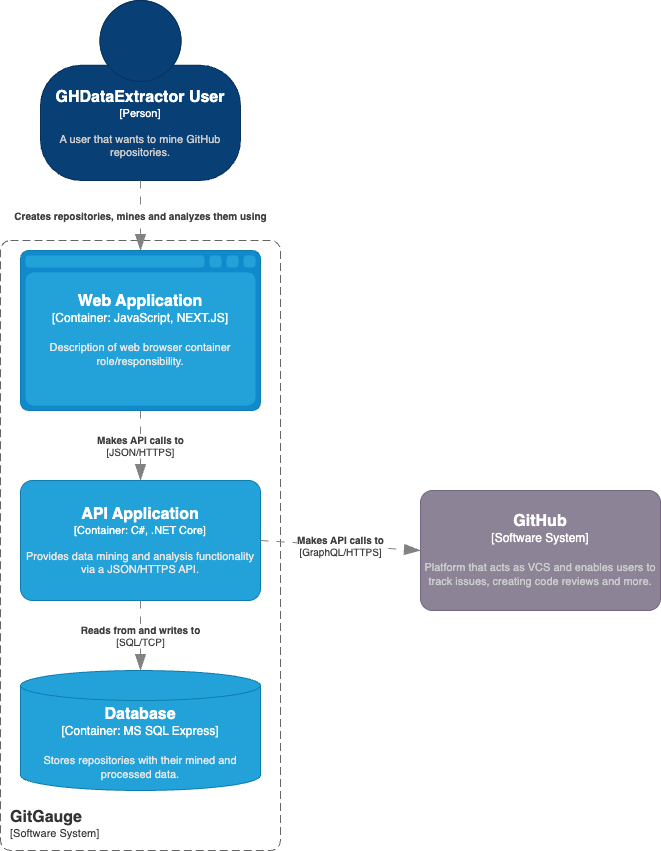
\includegraphics[width=0.8\textwidth]{Figures/container-diagram-gitgauge.png}
    \caption{Container Diagramm GitGauge \parencite{grand_joel_vt1_joelgrand_repository_2024}}
    \label{fig:container-diagram-gitgauge}
\end{figure}

Das \textit{Frontend} ist eine Next.js Webapplikation. Die Benutzer können über die Oberfläche neue Repositories hinzufügen und anschliessend den Mining-Prozess starten. Der Mining-Prozess kann auch jederzeit wiederholt werden. Anschliessend werden alle verfügbaren Metriken dargestellt. Die Wahl fiel auf Next.js, da dies serverseitiges Rendering unterstützt. Dies verbessert die Performance und erleichtert das Fetching der Daten. \parencite{grand_joel_vt1_joelgrand_repository_2024}

Das \textit{Backend} ist eine REST-API, welche in C\# mit Hilfe von \textit{.NET Core} implementiert wurde. Das Backend-Projekt ist in zwei Projekte unterteilt: dem Kernprojekt für die Hauptlogik und einem Data-Projekt, das als Object-Relational Mapping (ORM) Schicht die Datenschemata definiert. Intern folgt das Backend einer geschichteten Architektur mit klar getrennten Verantwortlichkeiten. Von den Controller-Klassen (für die REST-API) über Services (Businesslogik) bis zur Datenzugriffsschicht (Data Store). \parencite{grand_joel_vt1_joelgrand_repository_2024}

Die \textit{Datenbank} speichert sämtliche Daten, welche über die Projekte gesammelt wurden. Als Datenbank wird ein MSSQL-Server 2019 eingesetzt. \parencite{grand_joel_vt1_joelgrand_repository_2024}

\subsection{Repository Mining}
Das Mining der Daten wird in GitGauge mittels einer \textit{Mining Pipeline} abgebildet. Wie in \autoref{fig:overview-mining-steps} ersichtlich, besteht das Minen aus folgenden Phasen: Datenextraktion, Datenverarbeitung und Datenanalyse. 
In der Datenextraktionsphase werden alle relevanten Informationen aus dem GitHub-Repository ermittelt. Dabei werden 3 zentrale Datenquellen verwendet: Commits, Issues und PRs. Für das Analysieren der Commits wird mittels der Bibliothek LibGit2Sharp das Repository geklont. Dadurch können eventuelle API-Beschränkungen (Rate Limits) reduziert oder umgangen werden. Die Issues und PRs werden über die GraphQL-API von GitHub abgefragt. Im Vergleich zur klassischen REST-API performte die GraphQL-API deutlich besser, auch schon bei kleineren Projekten.  

In der Verarbeitungsphase werden die rohen GitHub-Daten bereinigt, gefiltert und in ein Analyseschema überführt. So werden fehlende Werte substituiert und die Daten normalisiert. 
Die Analyse der Daten erfolgt jeweils bei Abfrage der Statistik-API-Endpunkte des Backends. 

\begin{figure}[htbp]
    \centering
    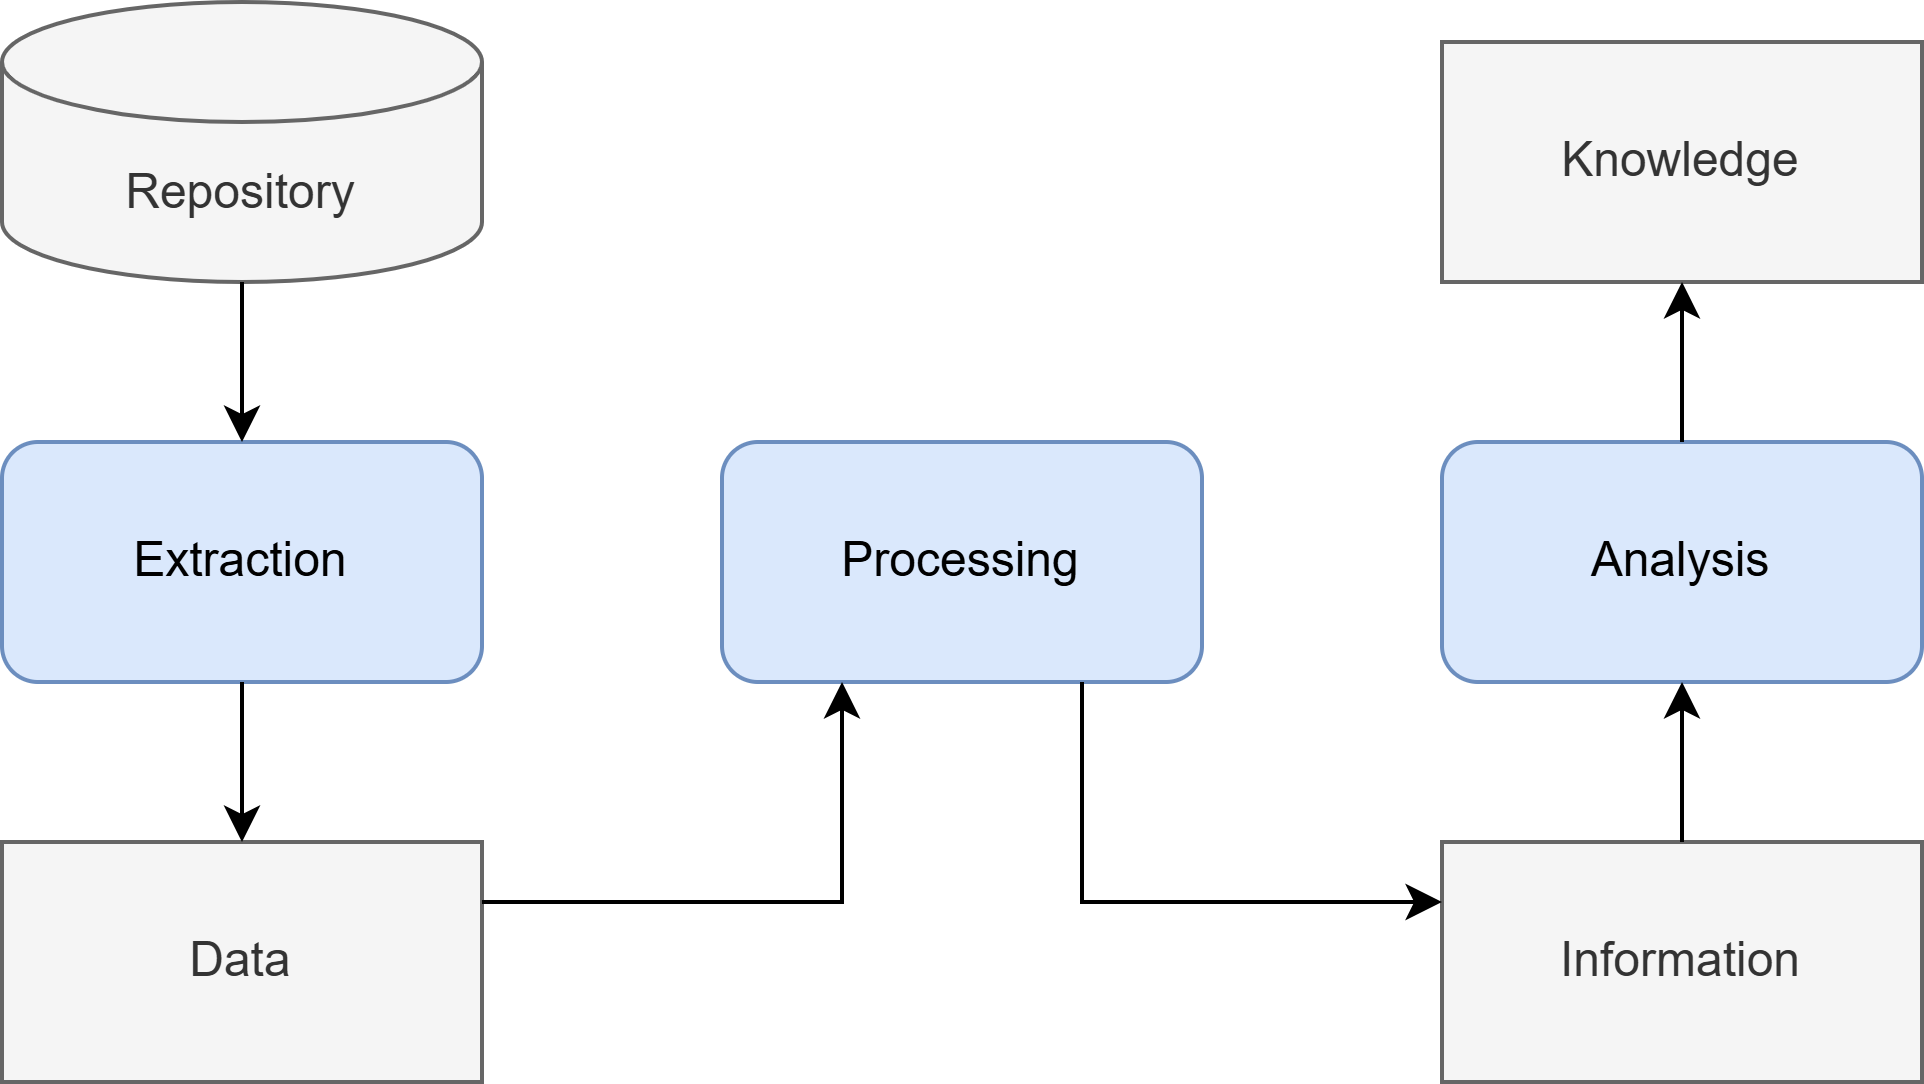
\includegraphics[width=0.8\textwidth]{Figures/uebersicht-mining-prozess.png}
    \caption{Übersicht Mining Prozess \parencite{grand_joel_vt1_joelgrand_repository_2024}}
    \label{fig:overview-mining-steps}
\end{figure}


